\label{speed_ratio}

Target survival is guaranteed if there is an overlapping of the region reachable by the Target before the Attacker (the interior of the $TA$ Apollonius circle) and the region $R_r$ reachable by the Defender before the Attacker (Fig. \ref{Rr2}), since within this overlapping, the Defender can perform its intended role of intercepting the Attacker before the Attacker captures the Target. Target survival is critical when the aforementioned overlapping diminishes into a single point at which the aforementioned two regions barely touch, or are tangent to one another.
For this situation, the normalized Target speed (the speed ratio) $\alpha=\dfrac{V_{T}}{V_{A}}$ attains its minimal or critical value $\overline{\alpha}$. Now, we consider three cases, in which the $TA$-Apollonius circle is tangent from outside to the boundary of the shaded region $R_r$. An implicit assumption throughout the forthcoming analysis is that $\boldsymbol{T}=(x_T , Y_T)$ is outside $R_r$. 

\section{The case $\gamma<1$ (fast defender)}
The critical speed ratio $\overline{\alpha}$, occurs when the $TA$ Apollonius circle is \textit{internally} tangent to the $AD$ Apollonius circle, i.e., when the centers $\boldsymbol{O_{2}}$ and $\boldsymbol{O_{1}}$ of these two circles and their tangency point $\boldsymbol{C}$ are collinear (Fig. \ref{4_g<1}). This happens when
\begin{equation}
r_{1}-r_{2}=\lvert\boldsymbol{O_{1}}-\boldsymbol{O_{2}}\rvert.
\label{dr_fd}
\end{equation}
Substituting for $r_{1}$,$r_{2}$,$\boldsymbol{O_1}$and $\boldsymbol{O_{2}}$ from (\ref{r1}), (\ref{r2}), (\ref{O1}) and (\ref{O2}) respectively, and noting that $\gamma<1$, one obtains

\begin{equation}
\begin{split}
\dfrac{2\gamma}{1-\gamma^{2}}x_{A}-\dfrac{\alpha}{1-\alpha^{2}}d 
&=\lvert(\dfrac{1+\gamma^{2}}{1-\gamma^{2}}x_{A},0)-\dfrac{1}{1-\alpha^{2}}(x_{T}-\alpha^{2}x_{A},y_{T})\rvert\\
&=[(\dfrac{1+\gamma^{2}}{1-\gamma^{2}}x_{A}-\dfrac{1}{1-\alpha^{2}}(x_{T}-\alpha^{2}x_{A}))^{2}+\dfrac{1}{(1-\alpha^{2})^{2}}y_{T}^2]^{\dfrac{1}{2}}.
\end{split}
\label{generaleq}
\end{equation}

In (\ref{generaleq}), we deliberately replaced $\lvert1-\gamma^{2}\rvert$ by $(1-\gamma^{2})$ because $\gamma<1$.
We now square both sides of (\ref{generaleq}) to obtain:

\begin{equation}
\begin{split}
\dfrac{4\gamma^{2}}{(1-\gamma^{2})^{2}}x_{A}^{2}
+\dfrac{\alpha^{2}}{(1-\alpha^{2})^{2}} d^{2}
-\dfrac{4\gamma\alpha d}{(1-\gamma^{2})(1-\alpha^{2})}x_{A}=\\
=\dfrac{(1+\gamma^{2})^{2}}{(1-\gamma^{2})^{2}}x_{A}^{2}
+\dfrac{x_{T}^{2}-2\alpha^{2} x_{T} x_{A}+\alpha^{4} x_{A}^{2} }{(1-\alpha^{2})^{2}}
-\dfrac{2(1+\gamma^{2})(x_{T}-\alpha^{2}x_{A})x_{A}}{(1-\gamma^{2})(1-\alpha^{2})}
+\dfrac{1}{(1-\alpha^{2})^{2}}y_{T}^{2}.
\end{split}
\label{generaleq2}
\end{equation}

By squaring both sides of equation (\ref{generaleq}), the cardinality of the solution set for equation (\ref{generaleq}) is doubled. This means that when we solve the resulting equation, half of the resulting solutions will be extraneous or irrelevant and have to be rejected. Fortunately, we will have genuine reasons that enable us to identify such solutions, and compel us to reject them. The solutions retained after such a rejection are the correct solutions of (\ref{dr_fd})
We now use (\ref{d}) to replace $y_{T}^{2}$ by $(d^{2}-x_{A}^{2}-x_{T}^{2}-2x_{A}x_{T})$ and rearrange terms in (\ref{generaleq2}) to obtain

\begin{equation}
\begin{split}
[\dfrac{4\gamma^{2}}{(1-\gamma^{2})^{2}}-\dfrac{(1+\gamma^{2})^{2}}{(1-\gamma^{2})^{2}}-\dfrac{\alpha^{4}}{(1-\alpha^{2})^{2}}-\dfrac{2\alpha^{2}(1+\gamma^{2})}{(1-\gamma^{2})(1-\alpha^{2})}+\dfrac{1}{(1-\alpha^{2})^{2}}]x_{A}^{2}\\
+[\dfrac{\alpha^{2}}{(1-\alpha^{2})^{2}}- \dfrac{1}{(1-\alpha^{2})^{2}}]d^{2}\\
-\dfrac{4\gamma\alpha x_{A}d}{(1-\gamma^{2})(1-\alpha^{2})}
+[\dfrac{-1}{(1-\alpha^{2})^{2}}+\dfrac{1}{(1-\alpha^{2})^{2}}]x_{T}^{2}\\
+[\dfrac{2\alpha^{2}}{(1-\alpha^{2})^{2}}+\dfrac{2(1+\gamma^{2})}{(1-\gamma^{2})(1-\alpha^{2})}-\dfrac{2}{(1-\alpha^{2})^{2}}]x_{T}x_{A}=0
\end{split}
\label{generaleq33}
\end{equation}


The coefficient of $x_A^2$ in (\ref{generaleq33}) is
\begin{equation}
\begin{split}
&\dfrac{4\gamma^{2}}{(1-\gamma^{2})^{2}}-\dfrac{(1+\gamma^{2})^{2}}{(1-\gamma^{2})^{2}}-\dfrac{\alpha^{4}}{(1-\alpha^{2})^{2}}-\dfrac{2\alpha^{2}(1+\gamma^{2})}{(1-\gamma^{2})(1-\alpha^{2})}+\dfrac{1}{(1-\alpha^{2})^{2}}\\
&=\dfrac{4\gamma^{2}-1-\gamma^{4}-2\gamma^2}{(1-\gamma^2)^2} + \dfrac{(1-\alpha^4)}{(1-\alpha^2)^2} - \dfrac{2\alpha^{2}(1-\gamma^2)}{(1-\gamma^2)(1-\alpha^2)}\\
&=-1 + \dfrac{1+\alpha^2}{(1-\alpha^2)}- \dfrac{2 \alpha^2 (1+\gamma^2)}{(1-\gamma^2)(1-\alpha^2)}\\
&= \dfrac{2\alpha^2}{(1-\alpha^2)} - \dfrac{2 \alpha^2 (1+\gamma^2)}{(1-\gamma^2)(1-\alpha^2)}\\
&= \dfrac{2 \alpha^2}{(1-\alpha^2)}[1-\dfrac{(1+\gamma^2)}{(1-\gamma^2)}] = \dfrac{2\alpha^2}{(1-\alpha^2)}(\dfrac{-2\gamma^2}{(1-\gamma^2)})\\
&= \dfrac{-4 \alpha^{2} \gamma^2}{(1-\alpha^2)(1-\gamma^2)},
\end{split}
\end{equation}

and the coefficient of $d^2$ in (\ref{generaleq33}) is
\begin{equation}
\dfrac{\alpha^{2}}{(1-\alpha^{2})^{2}}- \dfrac{1}{(1-\alpha^{2})^{2}}
= \dfrac{-(1-\alpha^2)}{(1-\alpha^2)^2} = -\dfrac{1}{(1-\alpha^2)},
\end{equation}

while the coefficient of $x_T x_A$ in (\ref{generaleq33}) is 

\begin{equation}
\begin{split}
&\dfrac{2\alpha^{2}}{(1-\alpha^{2})^{2}}+\dfrac{2(1+\gamma^{2})}{(1-\gamma^{2})(1-\alpha^{2})}-\dfrac{2}{(1-\alpha^{2})^{2}}\\
&= \dfrac{2(\alpha^{2}-1)}{(1-\alpha^2)^2} + \dfrac{2(1+\gamma^2)}{(1-\gamma^2)(1-\alpha^2)}\\
&= -\dfrac{2}{(1-\alpha^2)} + \dfrac{2(1+\gamma^2)}{(1-\gamma^2)(1-\alpha^2)}\\
&=\dfrac{2}{(1-\alpha^2)}[-1 + (\dfrac{1+\gamma^2}{1-\gamma^2})] = \dfrac{2}{(1-\alpha^2)}(\dfrac{2\gamma^2}{1-\gamma^2})\\
&=\dfrac{4\gamma^2}{(1-\alpha^2)(1-\gamma^2)}
\end{split}
\end{equation}

This means that equation (\ref{generaleq33}) can be simplified considerably to the equivalent form

\begin{equation}
\dfrac{-4 \alpha^{2}\gamma^{2}}{(1-\alpha^{2})(1-\gamma^{2})}x_{A}^{2}
-\dfrac{1}{1-\alpha^{2}}d^{2}
-\dfrac{4\gamma\alpha x_{A}d}{(1-\gamma^{2})(1-\alpha^{2})}
+\dfrac{4\gamma^{2}}{(1-\alpha^{2})(1-\gamma^{2})}x_{T}x_{A}
\label{generaleq3}
\end{equation}

Now, we multiply (\ref{generaleq3}) by $[-(1-\alpha^{2})(1-\gamma^{2})]$ noting that $\alpha\neq1$ and $\gamma\neq1$, to obtain

\begin{equation}
(4\gamma^{2}x_{A}^{2})\alpha^{2} + (4\gamma x_{A}d)\alpha + (1-\gamma^{2})d^{2} - 4\gamma^{2} x_{T} x_{A}=0
\label{generaleq4}
\end{equation}


or equivalently 
\begin{equation}
\boxed{
\alpha^{2}+\dfrac{d}{\gamma x_{A}}\alpha +[(\dfrac{1-\gamma^{2}}{4\gamma^{2}})(\dfrac{d}{x_{A}})^{2}-\dfrac{x_{T}}{x_{A}}]=0}
\label{eq36in3}
\end{equation}

Equation (\ref{eq36in3}) is an improvement of equation (36) in \cite{garcia2015escape}.
while (\ref{eq36in3}) is a quadratic equation in $\alpha$, equation (36) in \cite{garcia2015escape} is a quartic in $\alpha$ that has the same  two roots of (\ref{eq36in3}) in addition to the two irrelevant roots $\alpha\mp1$. As a bonus, equation (\ref{eq36in3}) is written in a self-verifying dimensionless form.

\section{The case $\gamma=1$ (similar Defender)}
The critical speed ratio $\overline{\alpha}$ occurs when the $TA$ Apollonius circle touches the $L.H.S.$ of the $XY-$plane (Fig. \ref{4_g=1}), i.e., when
\begin{equation}
r_{2}= Absicessa\ of\ \boldsymbol{O_{2}}.
\end{equation} 
i.e., thanks to (\ref{O2}) and (\ref{r2}) when:
\begin{equation}
\dfrac{\alpha d}{1-\alpha^{2}}=\dfrac{x_{T}-\alpha^{2}x_{A}}{1-\alpha^{2}}.
\label{case3}
\end{equation}

Multiplying (\ref{case3}) by $(1-\alpha^{2})$ (thanks to the fact that $\alpha\neq1$), and rearranging, one obtains the following quadratic equation in $\alpha$
\begin{equation}
x_{A} \alpha^{2} + d \alpha - x_{T}=0,
\label{case3_SD}
\end{equation}

which is equation (12) in [3]. It is interesting to note that equation (\ref{case3}) is the special case ($\gamma=1$) of (\ref{eq36in3}), 
though (\ref{eq36in3}) was derived under the assumption $\gamma\neq1$.




\section{The case $\gamma>1$ (Slow Defender)}
The critical speed ratio $\overline{\alpha}$ occurs when the $TA$ Apollonius circle is \textit{externally} tangent to the $AD$ Apollonius circle, i.e., when the centre $\boldsymbol{O_{2}}$, the tangency point $\boldsymbol{C}$ and the centre $\boldsymbol{O_{1}}$ are collinear(Fig. \ref{4_g>1}), i.e., when 
\begin{equation}
r_{1}+r_{2}=\lvert\boldsymbol{O_{1}}-\boldsymbol{O_{2}}\rvert
\label{case2}
\end{equation}      

Since $\gamma>1$, we write
\begin{equation}
r_{1}+r_{2}=\dfrac{2\gamma}{\lvert1-\gamma^{2}\rvert}+\dfrac{\alpha}{1-\alpha^{2}}d=\dfrac{-2 \gamma}{1-\gamma^{2}}+\dfrac{\alpha}{1-\alpha^{2}}d.
\end{equation}

The above expression for $(r_1+r_2)$ is exactly the negative of $(r_1-r_2)$ in (\ref{generaleq}).
Hence, squaring of (\ref{case2}) results in (\ref{generaleq2}), and consequently lead to (\ref{generaleq33}) and (\ref{generaleq3}), and finally to (\ref{generaleq4}) and (\ref{eq36in3}).
Equation (\ref{eq36in3}) is thereby shown to hold for a slow Defender besides being true for a fast one.

\begin{figure}
\centering
\subfigure[$\gamma<1$]{\includegraphics[width=0.6\textwidth]{fig/drawing4_2a.pdf}\label{4_g<1}}
\quad
\subfigure[$\gamma=1$]{\includegraphics[width=0.6\textwidth]{fig/drawing4_2c.pdf}\label{4_g=1}}
\quad
\subfigure[$\gamma>1$]{\includegraphics[width=0.6\textwidth]{fig/drawing4_2b.pdf}\label{4_g>1}}
\caption{The critical speed ratio $\overline{\alpha}$ is obtained when the $TA$ Apollonius circle is tangent to the boundary of the shaded region $R_r$ which is the region reachable by the Defender befor the Attacker.}
\label{CSR}
\end{figure}


Therefore, we will use the quadratic formula (\ref{eq36in3}) for all values of $\gamma$, and will solve it to obtain $\overline{\alpha}$ for any $\gamma$ as 

\begin{equation}
\begin{split}
\overline{\alpha}&=\dfrac{1}{2}[-\dfrac{d}{\gamma x_{A}}
\pm[(\dfrac{d}{\gamma x_{A}})^{2}-4(\dfrac{1-\gamma^{2}}{4\gamma^{2}})(\dfrac{d}{x_{A}})^{2}+\dfrac{4x_{T}}{x_{A}}]^{1/2} ]\\
&= \dfrac{1}{2\gamma x_{A}} [-d \mp \gamma \sqrt{d^{2}+4 x_{T} x_{A}}]\\
&= \dfrac{1}{2 \gamma x_{A}} [- \sqrt{(x_{A}-x_{T})^{2} + y^{2}}+ \gamma \sqrt{(x_{A}+ x_{T})^{2}+y_{T}^{2}}]
\end{split}
\label{cr_alpha_3}
\end{equation}






Equation (\ref{cr_alpha_3}) was derived in \cite{garcia2015escape} for $\gamma<1$ and in \cite{pachter2014active} for $\gamma=1$, provided $x_{T}>0$. It is shown herein to hold for all values in $\gamma$, including $\gamma>1$. Note that $\overline{\alpha}$ is definitely nonnegative and hence the minus sign in the solution for $\overline{\alpha}$ is rejected. The question remains whether (\ref{cr_alpha_3}) yields a non-negative value for $\overline{\alpha}$ when the positive sign is chosen in (\ref{cr_alpha_3}). It could be argued that (\ref{cr_alpha_3}) should be used (with the positive sign, of course) as long as it yields a nonnegative value for  $\overline{\alpha}$, and otherwise  $\overline{\alpha}$ should be set to zero. For example, if $\gamma=1$ and $x_T<0$, equation (\ref{cr_alpha_3}) yields a negative value for $\overline{\alpha}$ which need to be rejected and replaced by zero. Physically, the situation ${\gamma=1, x_T<0}$ is one in which the Target is initially in the region reachable by the Defender before the Attacker, i.e., it is within the effective protection of the Defender, even if it does not move itself at all. Therefor, we rewrite (\ref{cr_alpha_3}) in the following dimensionless form:

\begin{equation}
\overline{\alpha} = \dfrac{1}{2 \gamma} [-\sqrt{(1-\dfrac{x_T}{x_A})^2 + (\dfrac{y_T}{x_A})^2}+ \gamma \sqrt{(1+\dfrac{x_T}{x_A})^2 + (\dfrac{y_T}{x_A})^2}\ ]
\label{dimensionless-alphaCR}
\end{equation} 
provided that 

\begin{equation}
\gamma\ \sqrt{(1+\dfrac{x_T}{x_A})^2 + (\dfrac{y_T}{x_A})^2}\ > \sqrt{(1-\dfrac{x_T}{x_A})^2 + (\dfrac{y_T}{x_A})^2}
\label{ineq}
\end{equation}
and whenever (\ref{ineq}) is not valid, we simply set
\begin{equation}
\overline{\alpha}=0.
\end{equation}


%Tables 4.1 to 4.3 list values of $\overline{\alpha}$ versus values of $(\dfrac{x_T}{x_A})$ and $(\dfrac{y_T}{x_A})$ for the specific $\gamma$ values of 0.8, 1, and 1.25.
%Figures \ref{alphaCRgamma=0.8} to \ref{alphaCRgamma=1.25} plot $\alpha$ as a function of $(\dfrac{x_T}{x_A})$ with $(\dfrac{y_T}{x_A})$ as a parameter for the specific $\gamma$ values of 0.8, 1.0, and 1.25 respectively.
%
%\begin{figure}[htb]
%\centering
%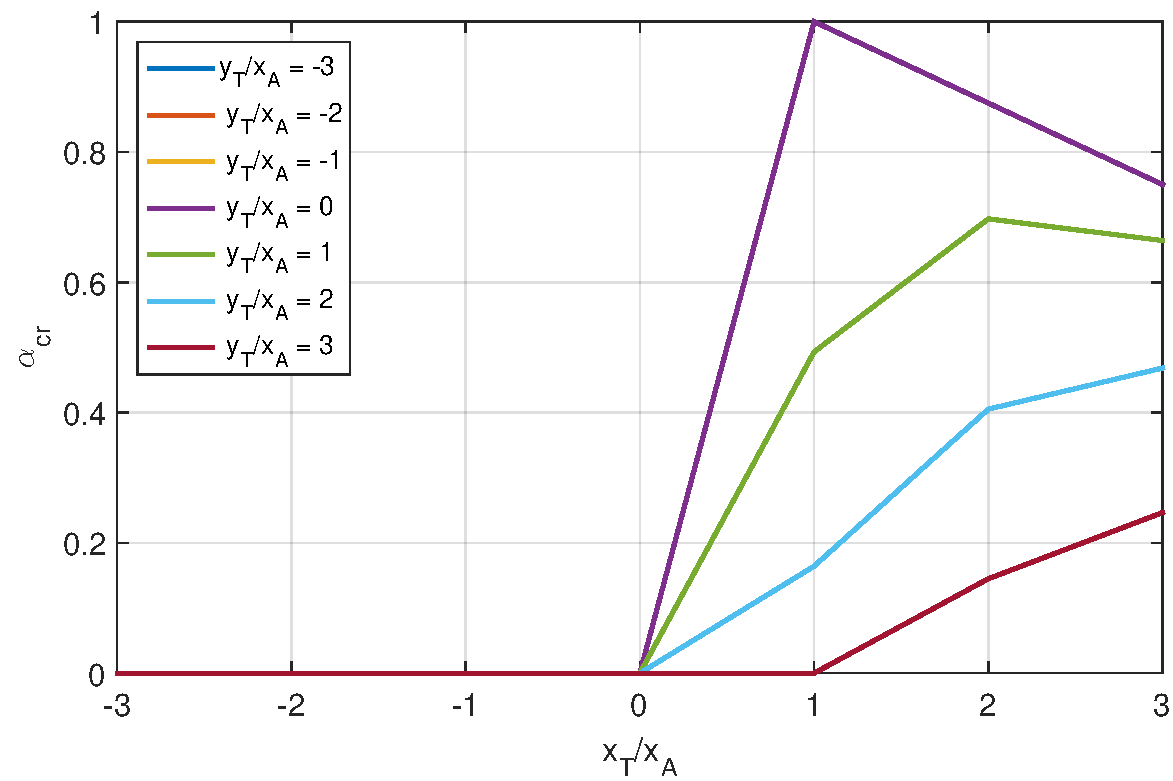
\includegraphics[scale = 0.6]{fig/alphaCRg_0p8.pdf}
%\caption{The critical normalized speed $\overline{\alpha}$ or $\alpha_{cr}$ as a function of $(\dfrac{x_T}{x_A})$ with $(\dfrac{y_T}{x_A})$ as a parameter when $\gamma=0.8$ (fast defender).}
%\label{alphaCRgamma=0.8}
%\end{figure}
%
%
%\begin{figure}[htb]
%\centering
%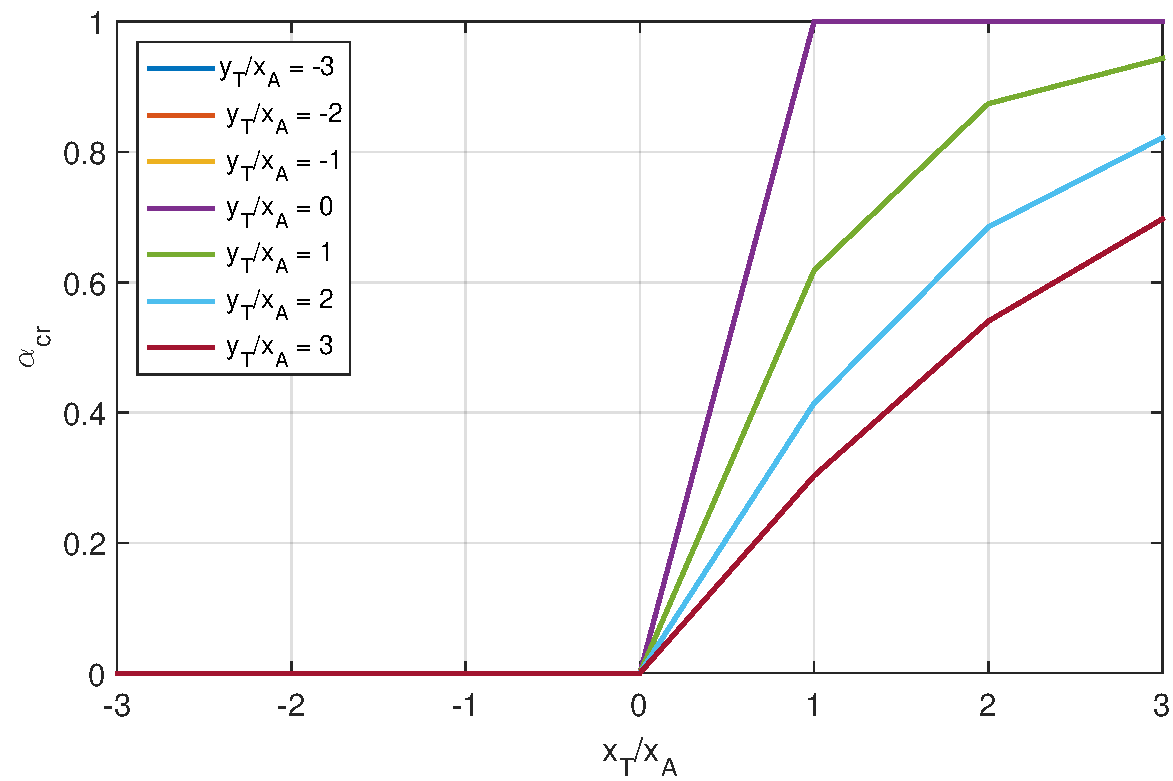
\includegraphics[scale = 0.6]{fig/alphaCRg_1.pdf}
%\caption{The critical normalized speed $\overline{\alpha}$ or $\alpha_{cr}$ as a function of $(\dfrac{x_T}{x_A})$ with $(\dfrac{y_T}{x_A})$ as a parameter when $\gamma=1$ (similar defender).}
%\label{alphaCRgamma=1}
%\end{figure}
%
%
%\begin{figure}[htb]
%\centering
%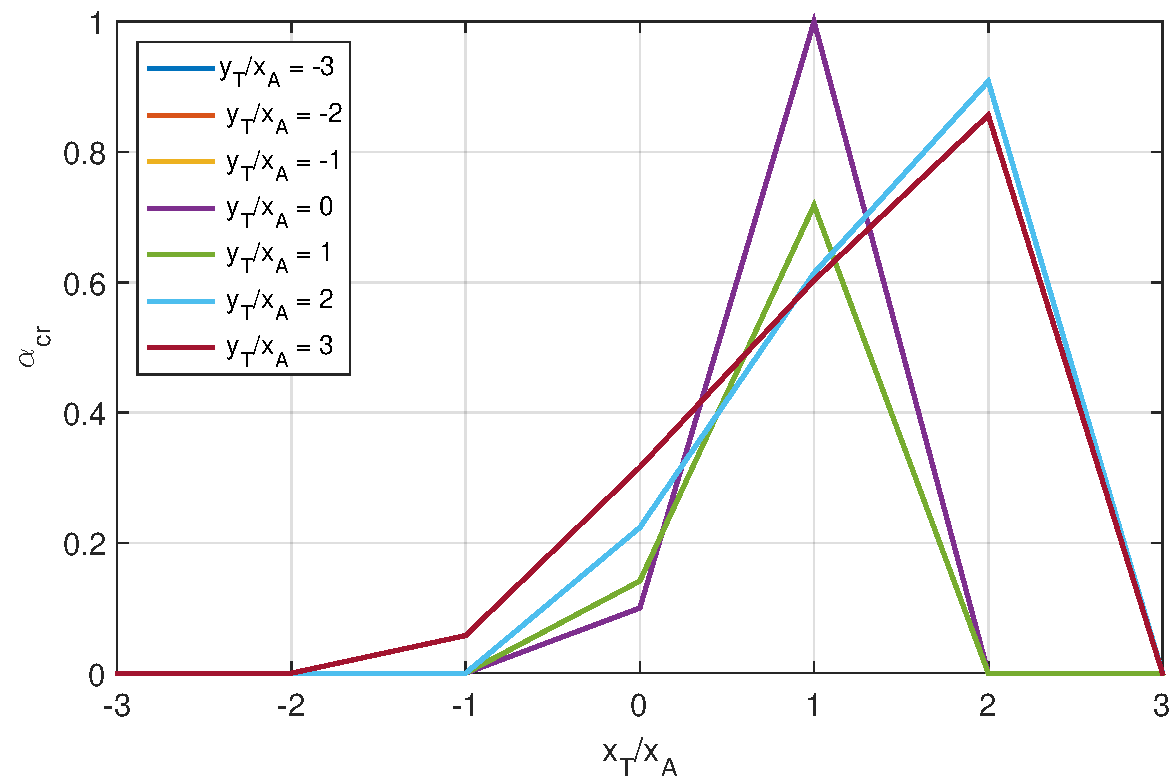
\includegraphics[scale = 0.6]{fig/alphaCRg_1p25.pdf}
%\caption{The critical normalized speed $\overline{\alpha}$ or $\alpha_{cr}$ as a function of $(\dfrac{x_T}{x_A})$ with $(\dfrac{y_T}{x_A})$ as a parameter when $\gamma=1.25$ (slow defender).}
%\label{alphaCRgamma=1.25}
%\end{figure}
%
%
%
%We pay a special attention to the special case when the Target is initially on the $x$-axis (i.e., when the Target, Attacker. and Defender are initially collinear). In this case, equation (\ref{dimensionless-alphaCR}) reduces to
%\begin{equation}
%\overline{\alpha} = \dfrac{1}{2 \gamma} [-\sqrt{(1-\dfrac{x_T}{x_A})^2}+ \gamma \sqrt{(1+\dfrac{x_T}{x_A})^2}\ ],
%\end{equation}
%care must be taken that the $\sqrt{\ }$ sign indicates the principal branch of the inverse square function. i.e., 
%\begin{equation}
%\sqrt{y^2} = \lvert y \rvert
%\end{equation}
%
%Therefore, we write
%\begin{equation}
%\sqrt{(1- \dfrac{x_T}{x_A})^2}=\begin{cases}
%1-\dfrac{x_T}{x_A},\ \ \ \ \ \dfrac{x_T}{x_A}\leq1\\
%\dfrac{x_T}{x_A}-1,\ \ \ \ \ \dfrac{x_T}{x_A}>1,
%\end{cases}
%\end{equation} 
%
%\begin{equation}
%\sqrt{(1+\dfrac{x_T}{x_A})^2}=\begin{cases}
%1+\dfrac{x_T}{x_A},\ \ \ \ \ \ \dfrac{x_T}{x_A}\geq-1\\
%-1-\dfrac{x_T}{x_A},\ \ \ \ \ \dfrac{x_T}{x_A}<-1,
%\end{cases}
%\end{equation}
%
%We now consider the three specific values of $\gamma$ considered in Figs. \ref{alphaCRgamma=0.8} to \ref{alphaCRgamma=1.25} , namely $\gamma=0.8, \gamma=1,$ and $\gamma=1.25$.\\
%
%
%\underline{\textbf{For $\gamma=0.8$}}
%\begin{equation}
%\overline{\alpha}= \dfrac{1}{1.6} [- \sqrt{(1-\dfrac{x_T}{x_A})^2}+ 0.8 \sqrt{(1+\dfrac{x_T}{x_A})^2}].
%\end{equation}
%For $(\dfrac{x_T}{x_A})<-1$\\
%
%\begin{center}
%$\overline{\alpha}=\dfrac{1}{1.6}[-(1-\dfrac{x_T}{x_A})+ 0.8(-1-\dfrac{x_T}{x_A})]
%=\dfrac{1}{1.6}[-1.8+0.2\dfrac{x_T}{x_A}]=\dfrac{1}{8}(-9+\dfrac{x_T}{x_A})$
%\end{center}
%
%which is definitely negative, and hence
%\begin{equation}
%\overline{\alpha}=0,\ \ \ \ \ (\dfrac{x_T}{x_A})<-1, \ \ \ \ \gamma=0.8
%\end{equation}
%
%For $-1\leq (\dfrac{x_T}{x_A})\leq 1$\\
%\begin{center}
%$\overline{\alpha}=\dfrac{1}{1.6}[-(1-\dfrac{x_T}{x_A})+0.8(1+\dfrac{x_T}{x_A})]= \dfrac{1}{1.6}[-0.2+1.8 \dfrac{x_T}{x_A}]= \dfrac{1}{8}(-1+9\dfrac{x_T}{x_A})$
%\end{center}
%The above $\overline{\alpha}$ is negative when $(-1+9 \dfrac{x_T}{x_A})$ is negative and hence we again set
%
%\begin{equation}
%\overline{\alpha}=0, \ \ \ \ \ -1\leq(\dfrac{x_T}{x_A})<\dfrac{1}{9}, \ \ \ \ \ \ \gamma=0.8.
%\end{equation}
%
%while $\overline{\alpha}$ increases linearly from 0 to 1 in $\dfrac{x_T}{x_A}\in [\dfrac{1}{9},1]$
%
%\begin{equation}
%\overline{\alpha} = \dfrac{1}{8} (-1 + 9 \dfrac{x_T}{x_A}), \ \ \ \ \ \dfrac{1}{9}\leq (\dfrac{x_T}{x_A})\leq 1, \ \ \ \ \ \gamma=0.8
%\end{equation}
%
%Finally, when $(\dfrac{x_T}{x_A})>1$
%\begin{equation}
%\overline{\alpha}= \dfrac{1}{1.6} [-(\dfrac{x_T}{x_A}-1)+ 0.8 (\dfrac{x_T}{x_A}+1)]
%=\dfrac{1}{1.6}[1.8 - 0.2 (\dfrac{x_T}{x_A})]
%=\dfrac{1}{8} (9-\dfrac{x_T}{x_A}).
%\end{equation}
%
%This means that after peaking at 1 when $(\dfrac{x_T}{x_A})=1$, the value of $\overline{\alpha}$ starts to decrease linearly to be 0 at $(\dfrac{x_T}{x_A})=9$ and then it remains 0 (rather than becoming negative), i.e.,
%\begin{equation}
%\overline{\alpha}=\dfrac{1}{8}(9-\dfrac{x_T}{x_A}), \ \ \ \ \ 1<(\dfrac{x_T}{x_A})\leq 9,\ \ \ \ \ \gamma=0.8,
%\end{equation}
%
%\begin{equation}
%\overline{\alpha}=0,\ \ \ \ \ (\dfrac{x_T}{x_A})>9,\ \ \ \ \ \gamma=0.8.
%\end{equation}
%
%
%\textbf{\underline{For $\gamma=1$}}
%
%\begin{equation}
%\overline{\alpha}= \dfrac{1}{2}[-\sqrt{(1-\dfrac{x_T}{x_A})^2}+ \sqrt{(1+\dfrac{x_T}{x_A})^2}\ ].
%\end{equation}
%
%For $(\dfrac{x_T}{x_A})<-1$\\
%\begin{center}
%$\overline{\alpha}= \dfrac{1}{2}[-(1-\dfrac{x_T}{x_A})+ (-1-\dfrac{x_T}{x_A})]=-1$.
%\end{center}
%
%Set
%\begin{equation}
%\overline{\alpha}=0,\ \ \ \ \ (\dfrac{x_T}{x_A})<-1,\ \ \ \ \ \gamma=1
%\end{equation}
%
%For $-1\leq (\dfrac{x_T}{x_A})\leq 1$\\
%\begin{center}
%$\overline{\alpha}=\dfrac{1}{2}[-(1-\dfrac{x_T}{x_A})+ (1+\dfrac{x_T}{x_A})]$
%\end{center}
%\begin{equation}
%\overline{\alpha}=(\dfrac{x_T}{x_A}),\ \ \ \ \ -1\leq(\dfrac{x_T}{x_A})\leq1,\ \ \ \ \ \gamma=1
%\end{equation}
%
%For $-1\leq(\dfrac{x_T}{x_A})<0$,  $\overline{\alpha}$ is again negative and is to be set to 0
%\begin{equation}
%\overline{\alpha}= (\dfrac{x_T}{x_A}),\ \ \ \ \ 0\leq(\dfrac{x_T}{x_A})\leq1,\ \ \ \ \ \gamma=1
%\end{equation}
%
%and hence $\overline{\alpha}$ increases linearly from 0 at $(\dfrac{x_T}{x_A})=0$ to 1 at $(\dfrac{x_T}{x_A})=1$
%
%For $(\dfrac{x_T}{x_A})>1$
%
%\begin{equation}
%\overline{\alpha} = \dfrac{1}{2} [-(\dfrac{x_T}{x_A}-1)+ (1+\dfrac{x_T}{x_A})]=1,\ \ \ \ \ (\dfrac{x_T}{x_A})>1,\ \ \ \ \ \gamma=1  
%\end{equation}
%
%Note that the situation of $(\gamma=1)$ differs significantly from that of $(\gamma=0.8)$. For $(\gamma=1)$, $\overline{\alpha}$ increases from 0 to 1 and remains so indefinitely, but for $(\gamma=0.8)$, $\overline{\alpha}$ increases from 0 to 1 and immediately decreases again to 0.\\
%
%
%\underline{\textbf{For $\gamma=1.25$}}
%\begin{equation}
%\overline{\alpha}= \dfrac{1}{2.5}[- \sqrt{(1-\dfrac{x_T}{x_A})^2}+ 1.25 \sqrt{(1+\dfrac{x_T}{x_A})^2}]
%\end{equation}
%
%For $(\dfrac{x_T}{x_A})<-1$
%\begin{center}
%$\overline{\alpha}=\dfrac{1}{2.5}[-(1-\dfrac{x_T}{x_A})+ 1.25 (-1-\dfrac{x_T}{x_A})]= \dfrac{1}{2.5}[-2.25-0.25\dfrac{x_T}{x_A}]=\dfrac{1}{10}(-9-\dfrac{x_T}{x_A}),$
%\end{center}
%
%which results in setting 
%\begin{equation}
%\overline{\alpha}=0,\ \ \ \ \ -9\leq(\dfrac{x_T}{x_A})<-1,\ \ \ \ \ \gamma=1.25,
%\end{equation}
%
%\begin{equation}
%\overline{\alpha}=\dfrac{1}{10}(-9-\dfrac{x_T}{x_A}),\ \ \ \ \ (\dfrac{x_T}{x_A})<-9,\ \ \ \ \ \gamma=1.25.
%\label{g=1.25,r<-1}
%\end{equation}
%
%For $-1\leq(\dfrac{x_T}{x_A})\leq1$
%\begin{center}
%$\overline{\alpha}=\dfrac{1}{2.5}[-(1-\dfrac{x_T}{x_A})+1.25(1+\dfrac{x_T}{x_A})]= \dfrac{1}{2.5}[0.25+2.25(\dfrac{x_T}{x_A})]=\dfrac{1}{10}[1+9\dfrac{x_T}{x_A}]$,
%\end{center}
%
%which reduces to 
%\begin{equation}
%\overline{\alpha}=0,\ \ \ \ \ -1\leq\dfrac{x_T}{x_A}<-\dfrac{1}{9},\ \ \ \ \ \gamma=1.25,
%\end{equation}
%
%\begin{equation}
%\overline{\alpha}=\dfrac{1}{10} (1+9 \dfrac{x_T}{x_A}),\ \ \ \ \ -\dfrac{1}{9}\leq\dfrac{x_T}{x_A}\leq1,\ \ \ \ \ \gamma=1.25.
%\end{equation}
%
%While $\overline{\alpha}$ remains 0 for $(\dfrac{x_T}{x_A})\in [-9,-\dfrac{1}{9})$ it starts to increase linearly to 1 for $(\dfrac{x_T}{x_A})\in[-\dfrac{1}{9},1)$.\\
%
%
%Finally, when $(\dfrac{x_T}{x_A})>1$
%\begin{equation}
%\overline{\alpha}=\dfrac{1}{2.5}[-(\dfrac{x_T}{x_A}-1)+ 1.25 (\dfrac{x_T}{x_A}+1)] = \dfrac{1}{2.5}[2.25+0.25 \dfrac{x_T}{x_A}]=\dfrac{1}{10}[9+\dfrac{x_T}{x_A}],
%\label{g=1.25,r>1}
%\end{equation}
%which means that $\overline{\alpha}$ increases linearly. Note that equations (\ref{g=1.25,r<-1}) and (\ref{g=1.25,r>1}) predict values of $\overline{\alpha}$ exceeding 1, a phenomenon taking place in the current analysis only when $\gamma>1$, i.e., for a slow defender. 

%======================================================
%\begin{figure}
%\centering
%\begin{subfigure}[b]{0.6\textwidth}
%\includegraphics[width=\textwidth]{drawing4_1a.pdf}
%\caption {$\gamma<1$}
%%\label{41_g<1}
%\end{subfigure}
%
%\begin{subfigure}[b]{0.6\textwidth}
%%\includegraphics[width=\textwidth]{\string"E:/Aero/Masters/guidance/paper2/documentation/fig/drawing4_1b\string".pdf}
%\includegraphics[width=\textwidth]{drawing4_1b.pdf}
%\caption {$\gamma=1$}
%%\label{41_g=1}
%\end{subfigure}
%
%\begin{subfigure}[b]{0.6\textwidth}
%%\includegraphics[width=\textwidth]{\string"E:/Aero/Masters/guidance/paper2/documentation/fig/drawing4_1c\string".pdf}
%\includegraphics[width=\textwidth]{drawing4_1c.pdf}
%\caption {$\gamma<1$}
%%\label{4_g>1}
%\end{subfigure}
%\caption{Shaded region $R_r$ is that reachable by the Defender befor the Atacker}
%\label{Rr}
%\end{figure}
